\documentclass[12pt,a4paper]{article}
\usepackage[a4paper,margin=1in]{geometry}
\usepackage{graphicx}
\usepackage{booktabs}
\usepackage{amsmath,amssymb}
\usepackage{float}
\usepackage{hyperref}
\usepackage{xcolor}
\usepackage{listings}
\usepackage{enumitem}
\usepackage{fancyhdr}
\usepackage{longtable}
\hypersetup{colorlinks=true,linkcolor=blue,urlcolor=blue}
\pagestyle{fancy}
\fancyhf{}
\lhead{ICS1512}
\rhead{Machine Learning Algorithms Laboratory}
\cfoot{\thepage}
\lstset{
language=Python,
basicstyle=\ttfamily\small,
numbers=left,
frame=single,
breaklines=true,
showstringspaces=false
}
\begin{document}

\begin{tabular}{|p{4cm}|p{11cm}|}
\hline
Experiment No. & 1 \\ \hline
Experiment Title & Exploratory Data Analysis on the Iris Dataset\footnote{\textbf{GitHub Repository: }\url{https://github.com/Harshitaab/ML_assignments_3122247001021}}\\ \hline
Student Name & Harshitaa B\\ \hline
Register Number & 3122247001021 \\ \hline
Faculty & Dr. Poreddy Ajay Kumar Reddy \\ \hline
Submission Date & 03-August-2026\\ \hline
\end{tabular}

\section{Objective}
The objective of this experiment is to perform a comprehensive Exploratory Data Analysis (EDA) on the Iris dataset using statistical summaries and visual representations. Specifically, the experiment aims to identify data distributions, detect missing values, and evaluate potential outliers across the continuous attributes of the dataset. In addition, the experiment assesses mathematical model assumptions such as normality, linearity, and multicollinearity among features, which in turn guide the choice of feature scaling techniques and the machine learning algorithms best suited to this data in subsequent experiments.

\section{Problem Statement}
The Iris dataset is a multivariate dataset consisting of morphological measurements of three species of the Iris flower. The problem addressed in this experiment is not classification itself, but the analysis that must precede it: given four continuous input features -- sepal length, sepal width, petal length, and petal width (all measured in centimetres) -- and a categorical output, the species class (\textit{Iris-setosa}, \textit{Iris-versicolor}, \textit{Iris-virginica}), the goal is to statistically and visually characterise the input space before any model is trained. This includes examining feature distributions, detecting missing data and outliers, and quantifying inter-feature correlation, so that appropriate preprocessing and modelling decisions can be justified rather than assumed.

\section{Dataset Description}
\begin{longtable}{|p{6cm}|p{8cm}|}
\hline
Dataset Name & Iris Dataset \\ \hline
Dataset Source & UCI Machine Learning Repository (\texttt{iris.csv}) \\ \hline
Number of Samples & 150 \\ \hline
Number of Features & 4 (sepal length, sepal width, petal length, petal width) \\ \hline
Number of Classes & 3 (\textit{Iris-setosa}, \textit{Iris-versicolor}, \textit{Iris-virginica}), 50 instances each \\ \hline
Missing Values & None (0 missing values across all 150 rows and 5 columns) \\ \hline
Train-Test Split & Not applicable at this stage; this experiment covers EDA only. A split (e.g. 80:20, stratified by class) will be introduced in the modelling experiment. \\ \hline
\end{longtable}

\section{Exploratory Data Analysis}

\subsection*{Dataset Overview}
The dataset was loaded using \texttt{pandas.read\_csv()} with explicit column names, since the raw file has no header row. It contains 150 rows and 5 columns -- four \texttt{float64} numerical features and one \texttt{object} categorical column (\texttt{class}). A check of the first five rows confirmed that the data loaded correctly, with values in the expected centimetre range and the label \textit{Iris-setosa} appearing for the initial records, consistent with the known ordering of the source file.

\subsection*{Statistical Summary}
The numerical statistics obtained via \texttt{df.describe()} are summarised below.

\begin{table}[H]
\centering
\begin{tabular}{lcccc}
\toprule
Statistic & Sepal Length & Sepal Width & Petal Length & Petal Width \\
\midrule
Count & 150 & 150 & 150 & 150 \\
Mean & 5.843 & 3.054 & 3.759 & 1.199 \\
Std. Dev. & 0.828 & 0.434 & 1.764 & 0.763 \\
Min & 4.300 & 2.000 & 1.000 & 0.100 \\
25\% & 5.100 & 2.800 & 1.600 & 0.300 \\
50\% (Median) & 5.800 & 3.000 & 4.350 & 1.300 \\
75\% & 6.400 & 3.300 & 5.100 & 1.800 \\
Max & 7.900 & 4.400 & 6.900 & 2.500 \\
\bottomrule
\end{tabular}
\caption{Descriptive statistics of the numerical features (all values in cm).}
\end{table}

The categorical summary of the \texttt{class} column shows 3 unique labels, with \textit{Iris-setosa} the most frequent, each of the three species occurring exactly 50 times -- confirming that the dataset is perfectly class-balanced.

Petal length and petal width show a much larger standard deviation relative to their mean than sepal length and sepal width, which is consistent with them varying sharply across the three species (as later confirmed by the bimodal histograms in Section 4.4).

\subsection*{Missing Value Analysis}

\begin{figure}[H]
\centering
\begin{figure}
    \centering
    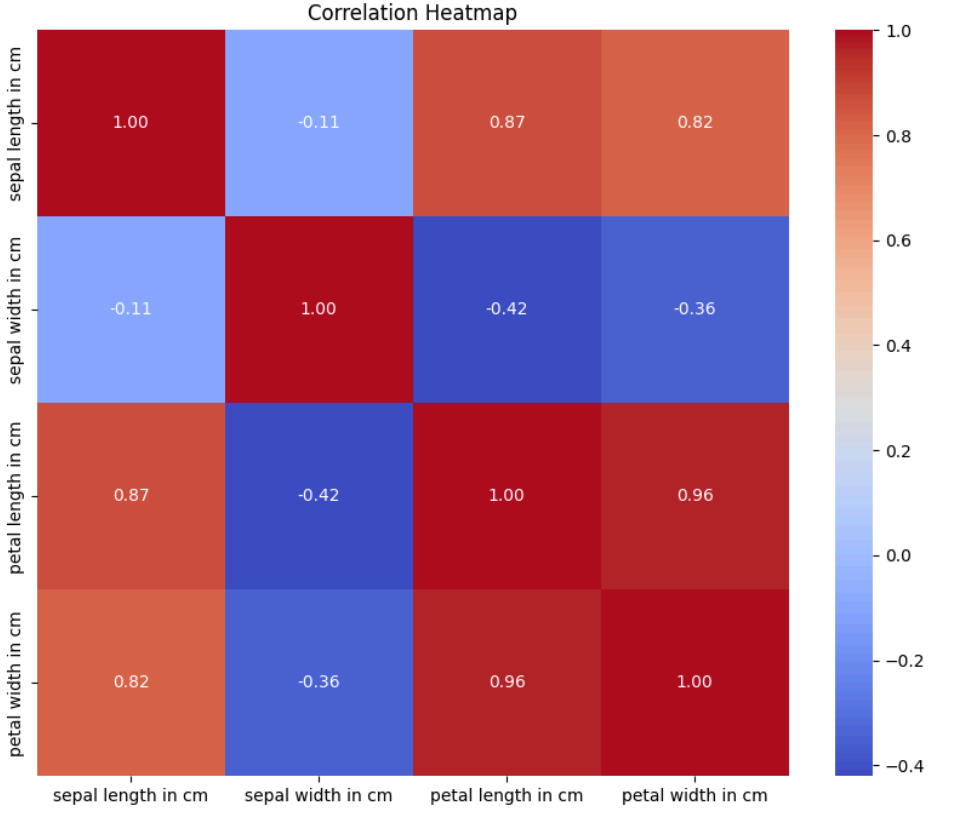
\includegraphics[width=0.75\linewidth]{corr_heatmap.png}
    \caption{Correlation matrix of missing values}
\begin{figure}
        \centering
        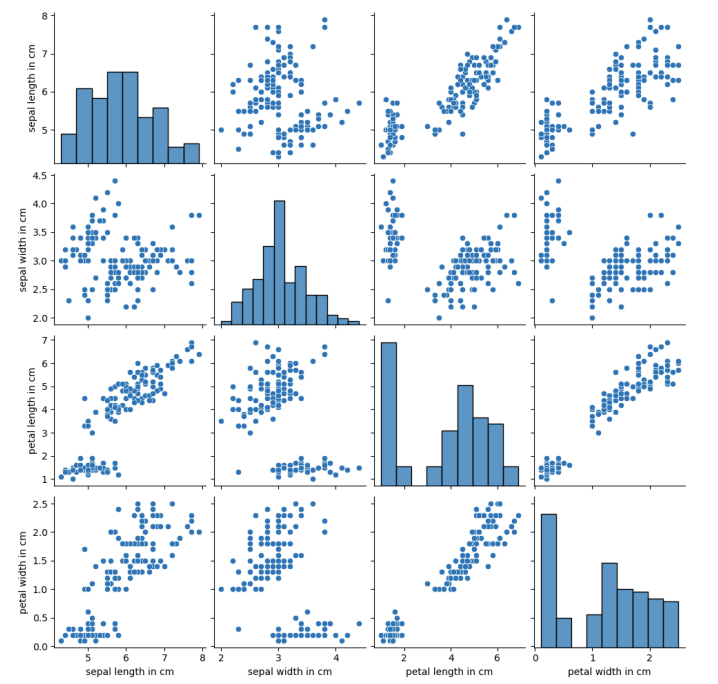
\includegraphics[width=0.75\linewidth]{pairplot.png}
        \caption{Pair plots of all the features present in the dataset}
        \label{fig:placeholder}
    \end{figure}
        \label{fig:placeholder}
\end{figure}
\begin{figure}
    \centering
    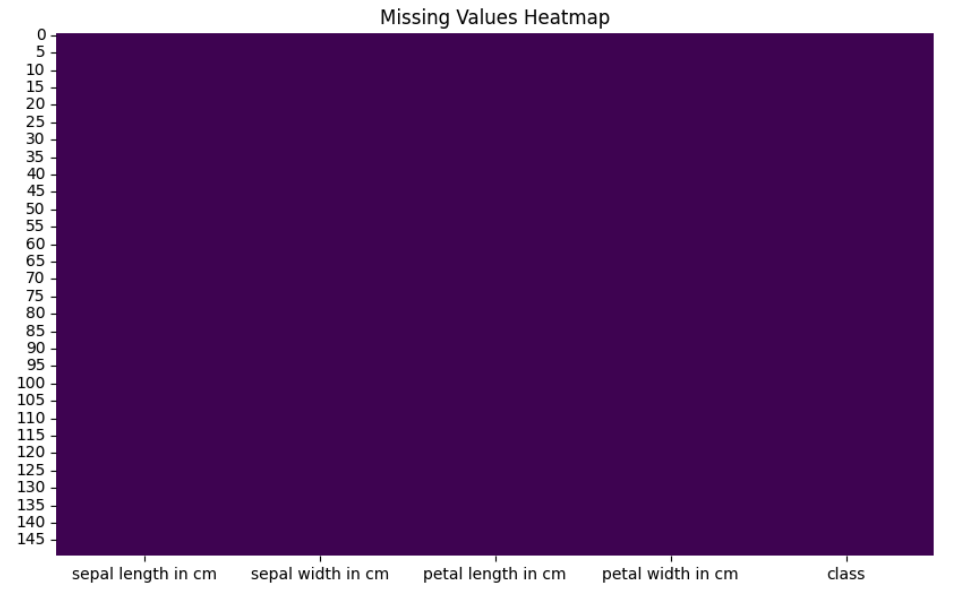
\includegraphics[width=0.5\linewidth]{missing_heatvalues.png}
    \caption{Enter Caption}
    \label{fig:placeholder}
\end{figure}
\caption{Missing values heatmap across all features of the Iris dataset.}
\end{figure}

\textbf{Inference:} The heatmap displays a single uniform colour across all 150 rows and 5 columns, with no contrasting cells that would indicate a missing entry. This visually confirms the result obtained from \texttt{df.isnull().sum()}, which reported a missing count and missing percentage of 0 for every column. Since the dataset is completely clean, no row deletion or imputation strategy (mean, median, mode, or KNN-based) is required prior to feature scaling or model training. This is expected, as the Iris dataset is a curated benchmark dataset rather than data collected from a live, error-prone source.

\subsection*{Class Distribution}
Although a dedicated count plot was not generated for this experiment, the categorical statistical summary (\texttt{df.describe(include='object')}) already establishes the class distribution: each of the three species -- \textit{Iris-setosa}, \textit{Iris-versicolor}, and \textit{Iris-virginica} -- accounts for exactly 50 of the 150 records. The dataset is therefore perfectly balanced, which means that accuracy will be a fair metric later during model evaluation and that no class-imbalance handling (e.g. class weighting, oversampling) will be necessary.

\subsection*{Correlation Matrix}

\begin{figure}[H]
\centering
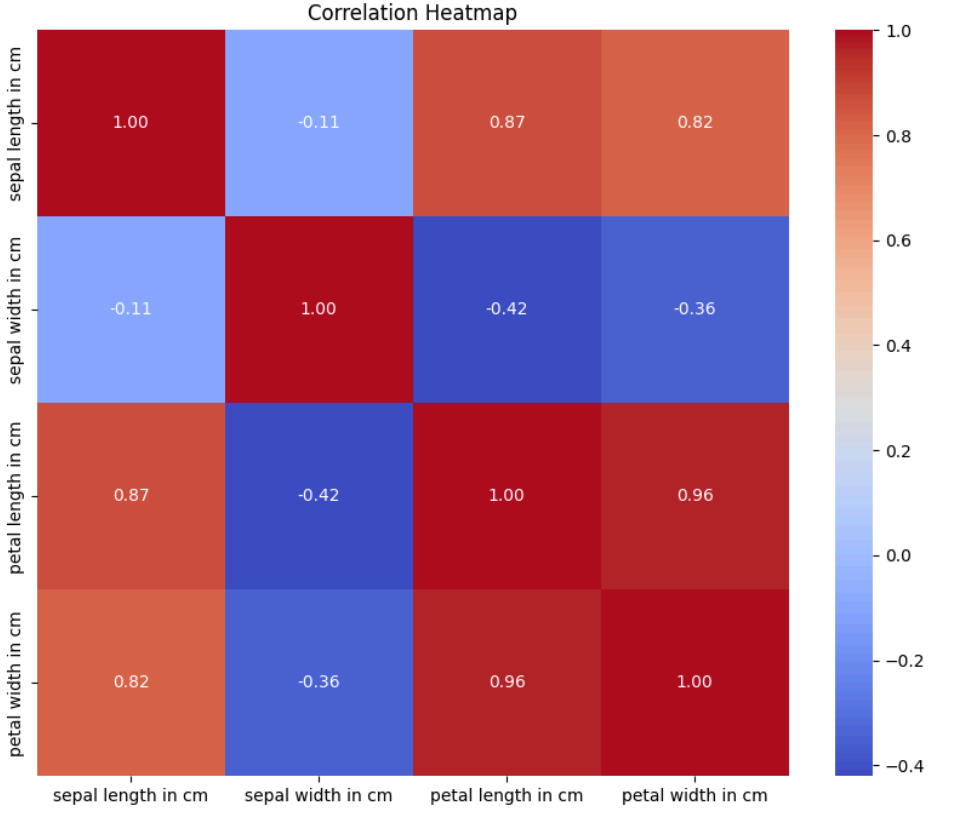
\includegraphics[width=0.75\linewidth]{corr_heatmap.png}
\caption{Pearson correlation heatmap of the four numerical features.}
\end{figure}

\textbf{Inference:} The correlation heatmap reveals strong positive linear relationships among several feature pairs. Petal length and petal width are almost perfectly correlated ($r = 0.96$), while sepal length correlates strongly with both petal length ($r = 0.87$) and petal width ($r = 0.82$). Sepal width, by contrast, shows weak or slightly negative correlation with the other three features. This high multicollinearity between the petal measurements suggests that they carry overlapping information, and that dimensionality reduction (e.g. PCA) or regularisation could be beneficial if a linear model is used downstream. The pair plot below reinforces this observation visually, showing that petal length and petal width also separate the three species almost linearly.

\begin{figure}[H]
\centering
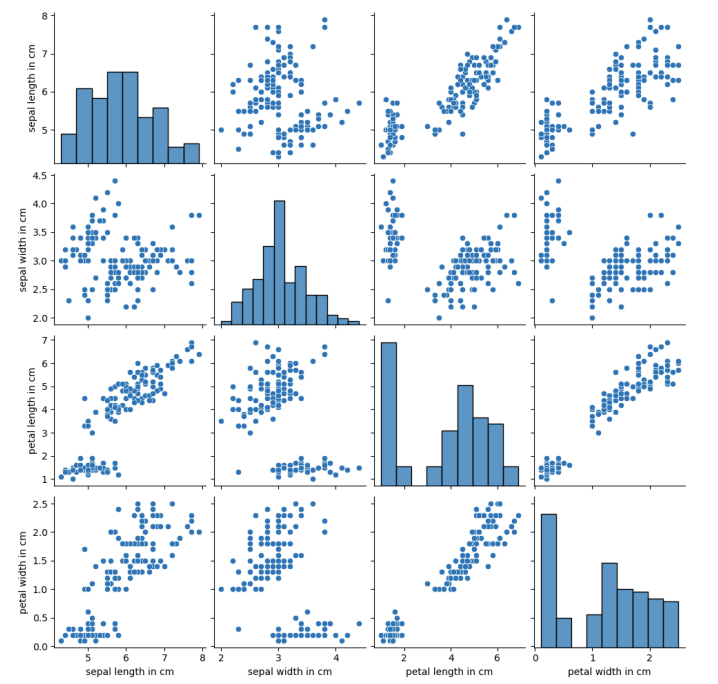
\includegraphics[width=0.85\linewidth]{pairplot.png}
\caption{Pairwise scatter plot matrix of the four numerical features.}
\end{figure}

\textbf{Inference:} The diagonal histograms and off-diagonal scatter plots show that \textit{Iris-setosa} is linearly separable from the other two species on almost every feature pair, particularly those involving petal length and petal width. \textit{Iris-versicolor} and \textit{Iris-virginica} overlap more, especially on the sepal measurements, indicating that a classifier will need the petal features to reliably distinguish between these two species.

\subsection*{Feature Distribution}

\begin{figure}[H]
\centering
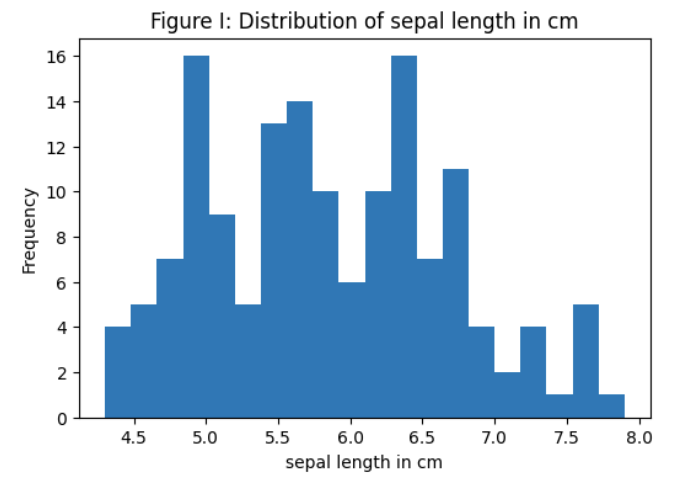
\includegraphics[width=0.6\linewidth]{hist_sepal_length.png}
\caption{Distribution of sepal length (cm).}
\end{figure}
\textbf{Inference:} The distribution is mildly bimodal, with peaks around 5.0~cm and 6.4~cm, and ranges from 4.3~cm to 7.9~cm. A skewness value of 0.31 indicates a slight right skew. The bimodality hints at underlying class structure, favouring non-linear or distance-based models over models that assume a single unimodal population.

\begin{figure}[H]
\centering
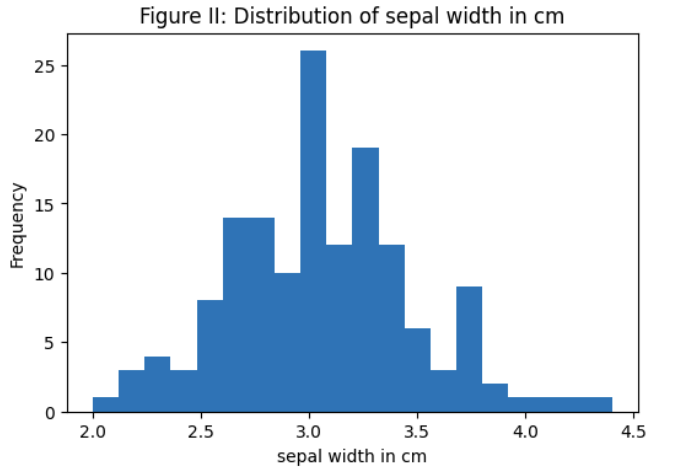
\includegraphics[width=0.6\linewidth]{hist_sepal_width.png}
\caption{Distribution of sepal width (cm).}
\end{figure}
\textbf{Inference:} Sepal width is the most symmetric of the four features (skewness $= 0.33$), showing an approximately normal, bell-shaped distribution centred near 3.0~cm and spread between roughly 2.0~cm and 4.4~cm. Because it best satisfies the normality assumption, this feature is best suited to standardisation ($\mu = 0, \sigma = 1$) if a model that assumes Gaussian-distributed inputs is used.

\begin{figure}[H]
\centering
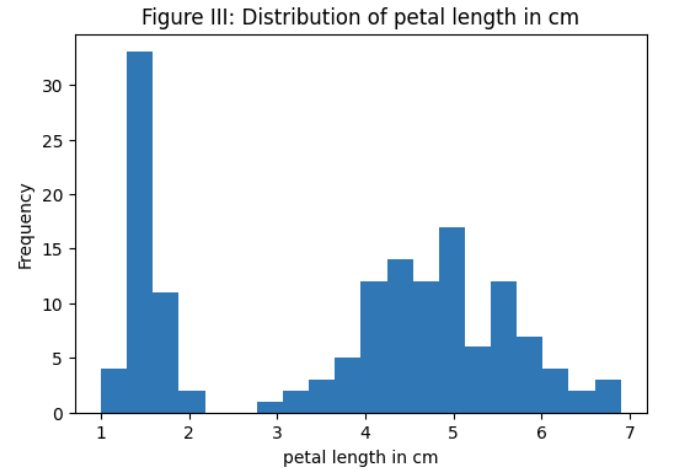
\includegraphics[width=0.6\linewidth]{hist_petal_length.png}
\caption{Distribution of petal length (cm).}
\end{figure}
\textbf{Inference:} Petal length shows a strongly bimodal distribution with a clear empty gap between 2.2~cm and 3.0~cm, separating a sharp low peak (1.0--1.8~cm, corresponding to \textit{setosa}) from a broader, higher cluster (3.0--6.9~cm, corresponding to \textit{versicolor} and \textit{virginica}). Skewness is $-0.27$. This clean separation makes petal length one of the most discriminative features for classification.

\begin{figure}[H]
\centering
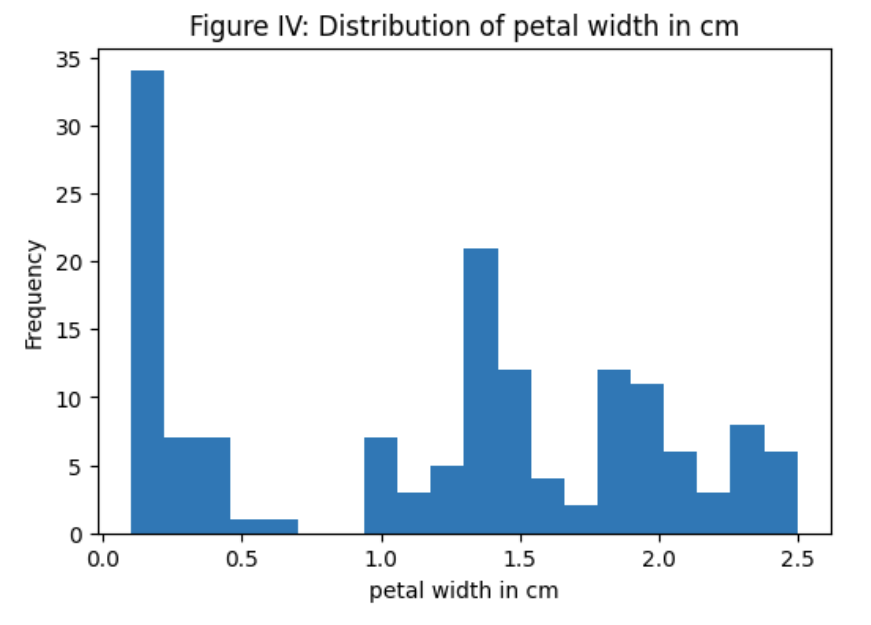
\includegraphics[width=0.6\linewidth]{hist_petal_width.png}
\caption{Distribution of petal width (cm).}
\end{figure}
\textbf{Inference:} Petal width mirrors petal length, with a pronounced gap between 0.7~cm and 0.9~cm separating a sharp low peak (0.1--0.4~cm) from a wider cluster (1.0--2.5~cm). With a near-zero skewness of $-0.10$, the distribution is the most balanced in shape among the four features despite its bimodality, and remains one of the two strongest discriminative features alongside petal length.

\subsection*{Outlier Analysis}
Boxplots and the IQR method ($x < Q_1 - 1.5 \times \text{IQR}$ or $x > Q_3 + 1.5 \times \text{IQR}$) were used to detect univariate outliers.

\begin{figure}[H]
\centering
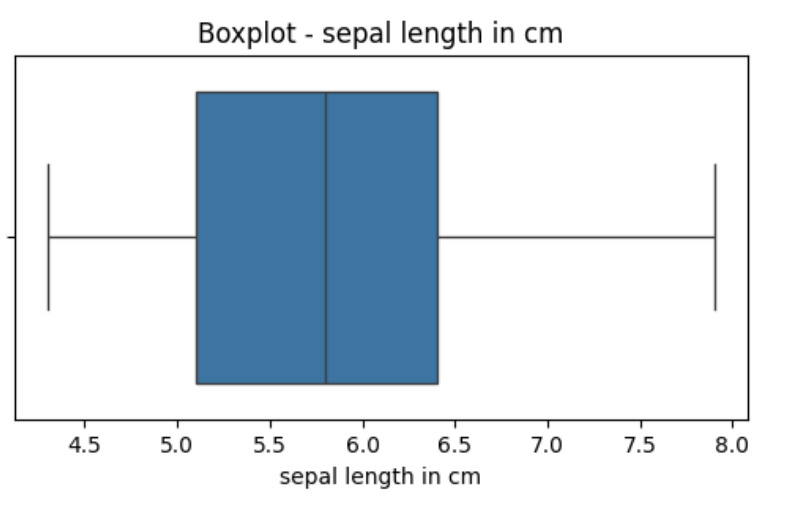
\includegraphics[width=0.55\linewidth]{box_sepal_length.png}
\caption{Boxplot of sepal length.}
\end{figure}
\textbf{Inference:} No outliers were detected (0 points beyond the whiskers). The median sits near 5.8~cm with the IQR spanning 5.1--6.4~cm, indicating a balanced spread with no extreme skew.

\begin{figure}[H]
\centering
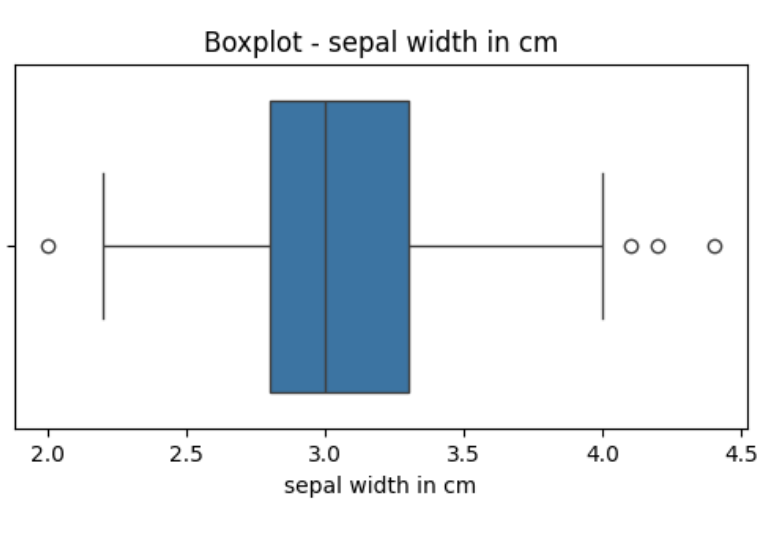
\includegraphics[width=0.55\linewidth]{box_sepal_width.png}
\caption{Boxplot of sepal width.}
\end{figure}
\textbf{Inference:} Sepal width is the only feature with detected outliers -- 4 points in total, one below $\approx 2.0$~cm and three above $\approx 4.1$--$4.4$~cm. These are retained rather than removed, since they fall within the natural biological range of the species and do not appear to be data-entry errors.

\begin{figure}[H]
\centering
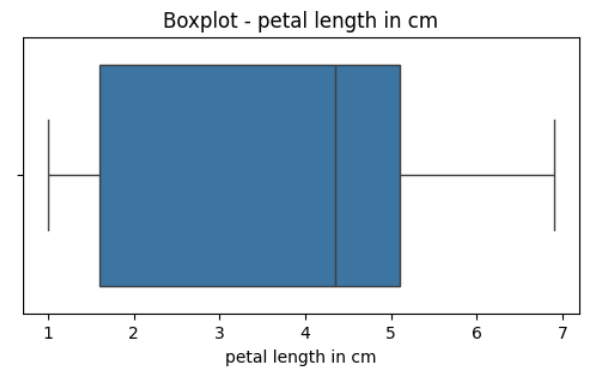
\includegraphics[width=0.55\linewidth]{box_petal_length.png}
\caption{Boxplot of petal length.}
\end{figure}
\textbf{Inference:} No outliers were detected. The median is shifted right ($\approx 4.35$~cm) with a wide IQR (1.6--5.1~cm), reflecting the presence of distinct species sub-clusters rather than a single centred distribution.

\begin{figure}[H]
\centering
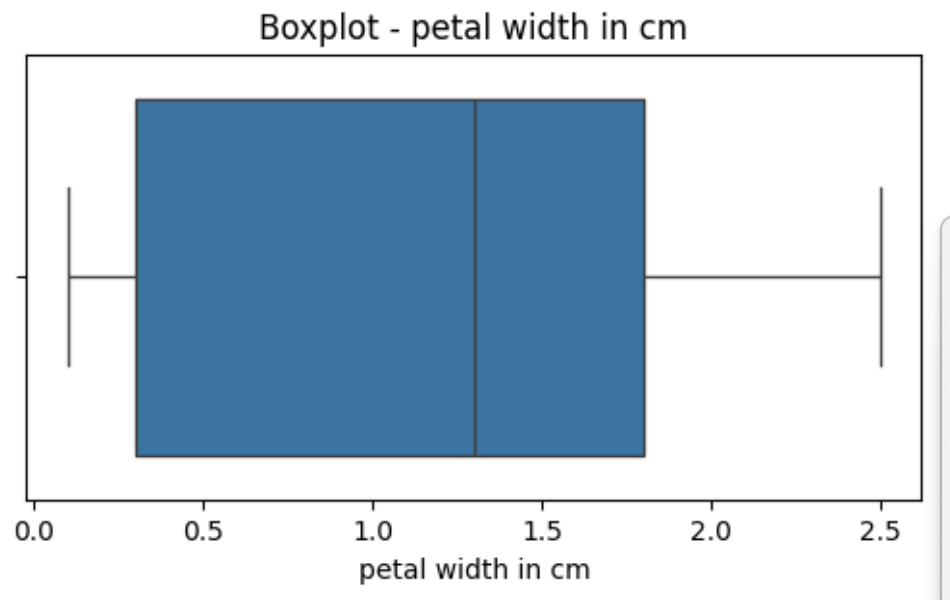
\includegraphics[width=0.55\linewidth]{box_petal_width.png}
\caption{Boxplot of petal width.}
\end{figure}
\textbf{Inference:} No outliers were detected. The median sits at $\approx 1.3$~cm with an IQR of 0.3--1.8~cm; a slightly longer upper whisker points to a mild right skew driven by the larger petal measurements of \textit{Iris-virginica}.

The IQR-based outlier report confirms these visual findings numerically: sepal length -- 0 outliers, sepal width -- 4 outliers, petal length -- 0 outliers, petal width -- 0 outliers.

\section{Data Preprocessing}
\textbf{Missing value handling:} Not required, since the missing-value analysis in Section 4 confirmed zero missing entries across all columns.

\textbf{Encoding:} The target column \texttt{class} is categorical with three labels. For downstream modelling, this will need to be label-encoded (e.g. \textit{Iris-setosa} $\to 0$, \textit{Iris-versicolor} $\to 1$, \textit{Iris-virginica} $\to 2$) using \texttt{sklearn.preprocessing.LabelEncoder}, since none of the four input features are categorical, only the target requires encoding.

\textbf{Feature scaling:} The four features are all measured in the same unit (cm) but on different scales (e.g. petal length ranges up to 6.9~cm, petal width only up to 2.5~cm). Sepal width is close to normally distributed and is therefore a good candidate for standardisation ($z = (x-\mu)/\sigma$), whereas sepal length, petal length, and petal width are bimodal rather than normal, so normalisation (min--max scaling to $[0,1]$) may be more appropriate for these if a distance-based algorithm such as KNN is used. In practice, since the strong multicollinearity identified in the correlation analysis affects distance-based and linear models similarly, standard scaling will be applied uniformly across all four features before model training, which is the more common convention for this dataset.

\textbf{Train-test split:} To be performed in the model-training experiment; an 80:20 stratified split (stratified on the class label to preserve the 50/50/50 balance) is recommended given the balanced, moderate-size dataset.

\textbf{Feature engineering:} Not applied in this experiment. Given the very high correlation between petal length and petal width ($r=0.96$), a derived ``petal area'' feature (length $\times$ width) could be explored as a candidate feature engineering step in future experiments, though it is not implemented here.

\section{Machine Learning Algorithm}
This experiment (Experiment 1) is restricted to Exploratory Data Analysis and does not train a classification model; therefore working principle, mathematical formulation, advantages, and limitations of a specific algorithm are not applicable here. Based on the EDA findings, however, the following observations will guide the algorithm choice in the next experiment: since \textit{Iris-setosa} is linearly separable from the other two species while \textit{versicolor} and \textit{virginica} overlap moderately, both simple linear classifiers (Logistic Regression, LDA) and distance-based / margin-based classifiers (KNN, SVM) are expected to perform well, with tree-based ensembles (Random Forest) serving as a strong non-linear baseline given the bimodal, cluster-like feature distributions observed above.

\section{Experimental Setup}
\begin{tabular}{ll}
\toprule
Python Version & 3.12.13\\
Scikit-Learn Version & \\
IDE & Google Colab \\
Operating System & Windows\\
Hardware & PC\\
\begin{figure}
    \centering
    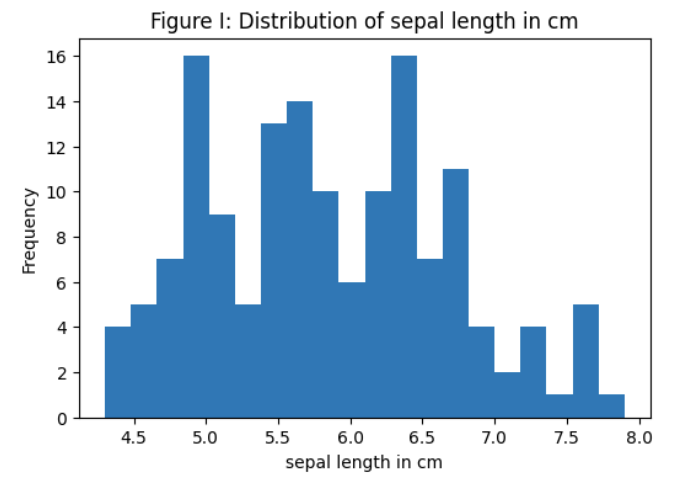
\includegraphics[width=0.75\linewidth]{hist_sepal_length.png}
    \caption{Enter Caption}
\begin{figure}
        \centering
        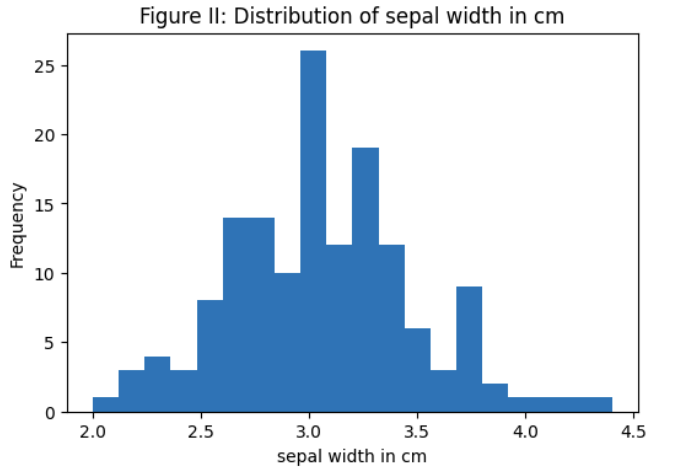
\includegraphics[width=0.75\linewidth]{hist_sepal_width.png}
        \caption{Enter Caption}
\begin{figure}
            \centering
            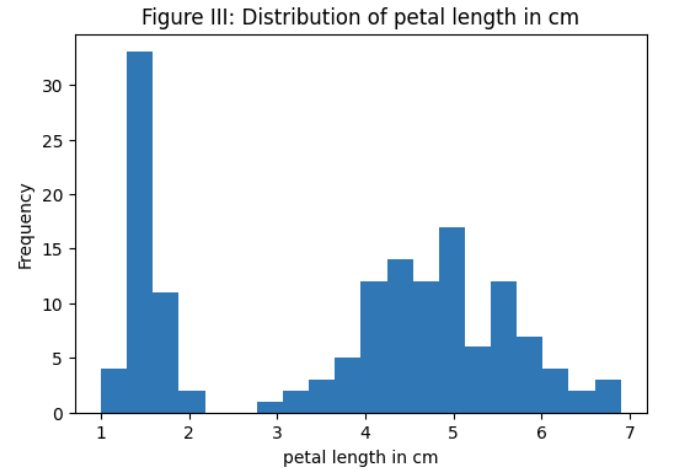
\includegraphics[width=0.75\linewidth]{hist_petal_length.png}
            \caption{Enter Caption}
\begin{figure}
                \centering
                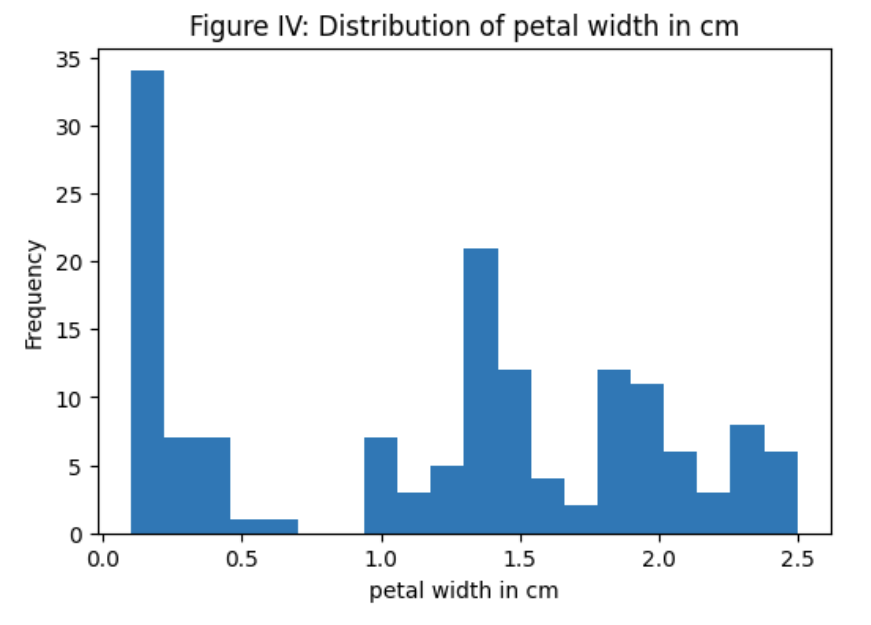
\includegraphics[width=0.75\linewidth]{hist_petal_width.png}
                \caption{Enter Caption}
\begin{figure}
                    \centering
                    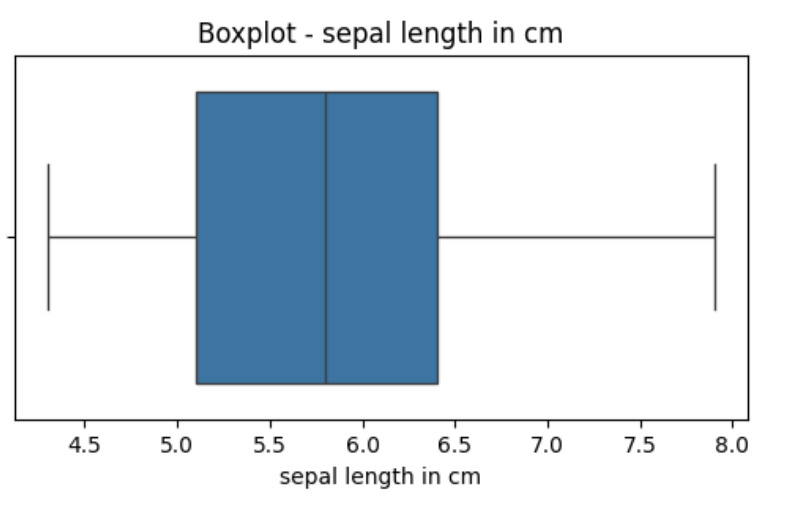
\includegraphics[width=0.75\linewidth]{box_sepal_length.png}
                    \caption{Enter Caption}
\begin{figure}
                        \centering
                        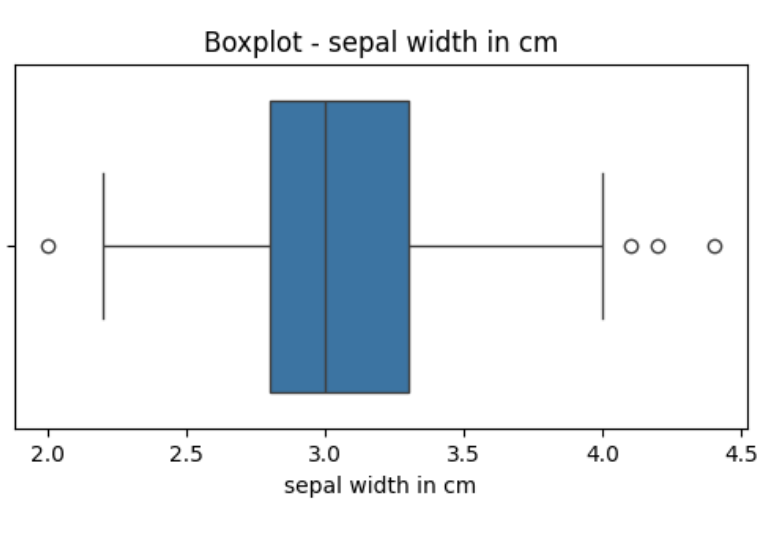
\includegraphics[width=0.75\linewidth]{box_sepal_width.png}
                        \caption{Enter Caption}
\begin{figure}
                            \centering
                            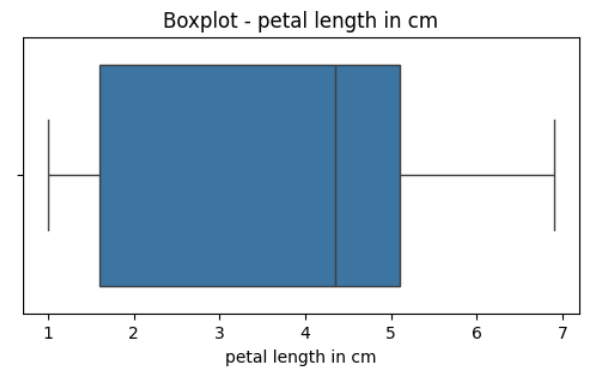
\includegraphics[width=0.75\linewidth]{box_petal_length.png}
                            \caption{Enter Caption}
\begin{figure}
                                \centering
                                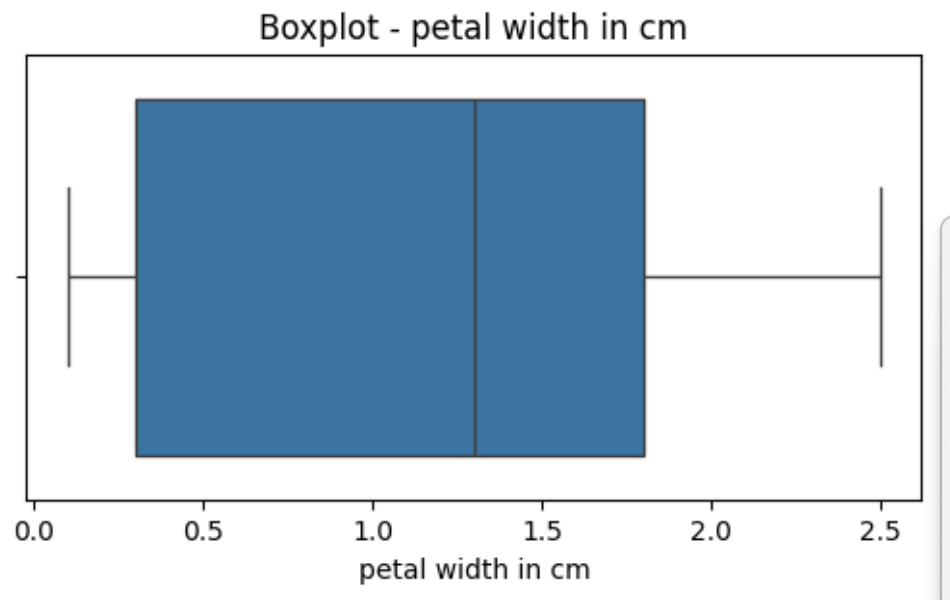
\includegraphics[width=0.75\linewidth]{box_petal_width.png}
                                \caption{Enter Caption}
                                \label{fig:placeholder}
                            \end{figure}
                                                        \label{fig:placeholder}
                        \end{figure}
                                                \label{fig:placeholder}
                    \end{figure}
                                        \label{fig:placeholder}
                \end{figure}
                                \label{fig:placeholder}
            \end{figure}
                        \label{fig:placeholder}
        \end{figure}
                \label{fig:placeholder}
    \end{figure}
        \label{fig:placeholder}
\end{figure}
\bottomrule
\end{tabular}



\section{Hyperparameter Selection}
Not applicable -- no model was trained in this EDA-only experiment.

\section{Results}
\begin{tabular}{lc}
\toprule
Metric & Value\\
\midrule
Accuracy & N/A \\
Precision & N/A \\
Recall & N/A \\
F1-score & N/A \\
ROC-AUC & N/A \\
\bottomrule
\end{tabular}

\textit{Note: These metrics are not applicable to Experiment 1, since it covers EDA only. They will be reported once a classifier is trained in the subsequent modelling experiment.}

\section{Result Visualization}
All plots generated during this experiment are Exploratory Data Analysis visualisations, and are presented in full with captions and inferences in Section 4 (missing-value heatmap, feature histograms, boxplots, correlation heatmap, and pair plot). Model-evaluation visualisations recommended by the template -- Confusion Matrix, ROC Curve, Precision-Recall Curve, Learning Curve, and Feature Importance -- are not applicable to this experiment, since no classifier has yet been trained; these will be produced and discussed in the modelling experiment that follows.

\section{Discussion}
The Iris dataset proved to be exceptionally clean: there were no missing values in any of the 150 records, and only sepal width exhibited any outliers (4 points, all within a biologically plausible range). The statistical summary and histograms showed that petal length and petal width are strongly bimodal and highly discriminative, cleanly separating \textit{Iris-setosa} from the other two species, whereas sepal width is the only feature that is close to normally distributed. The correlation analysis quantified what the pair plot suggested visually: petal length and petal width are almost collinear ($r=0.96$), and both correlate strongly with sepal length ($r=0.87$ and $r=0.82$ respectively), indicating redundancy among the petal- and length-related measurements.

A key strength of this dataset is its balance (50 samples per class) and completeness, which removes the need for imputation or class-imbalance correction and allows accuracy to be used as a fair evaluation metric later. A limitation is the small sample size (150 rows total, only 50 per class), which increases the variance of any train-test split and makes cross-validation preferable to a single held-out split for the next experiment. The multicollinearity identified between petal length and petal width also means that models sensitive to correlated inputs (e.g. plain linear regression coefficients) would need to be interpreted with caution, or that dimensionality reduction should be considered if interpretability of individual feature weights is required. Overall, the EDA strongly suggests that petal length and petal width will be the primary drivers of classification performance in the next stage.

\section{Conclusion}
This experiment carried out a complete Exploratory Data Analysis of the Iris dataset. The analysis confirmed that the dataset contains 150 samples across 3 balanced classes with 4 numerical features and no missing values. Distribution analysis revealed that petal length and petal width are strongly bimodal and highly discriminative between species, while sepal width is the only approximately normal feature and also the only one containing outliers under the IQR method. Correlation analysis exposed strong multicollinearity between the petal features and sepal length. These findings directly motivate the preprocessing plan (standard scaling of all features, label-encoding of the target, and an 80:20 stratified split) and the choice of candidate algorithms (linear, distance-based, and tree-based classifiers) to be evaluated in the subsequent classification experiment.

\section{References}
\begin{enumerate}[label={[\arabic*]}]
\item R. A. Fisher, ``The use of multiple measurements in taxonomic problems,'' \textit{Annals of Eugenics}, vol. 7, no. 2, pp. 179--188, 1936.
\item UCI Machine Learning Repository, ``Iris Data Set.'' [Online]. Available: \url{https://archive.ics.uci.edu/ml/datasets/iris}
\item W. McKinney, ``Data Structures for Statistical Computing in Python,'' in \textit{Proc. 9th Python in Science Conf.}, 2010, pp. 56--61.
\item M. L. Waskom, ``seaborn: statistical data visualization,'' \textit{Journal of Open Source Software}, vol. 6, no. 60, p. 3021, 2021.
\item J. D. Hunter, ``Matplotlib: A 2D Graphics Environment,'' \textit{Computing in Science \& Engineering}, vol. 9, no. 3, pp. 90--95, 2007.
\end{enumerate}
\documentclass{article}
\usepackage{hyperref}

\begin{document}

\section*{GitHub Link}
\url{https://github.com/Harshitaab/ML_assignments_3122247001021}

% OR if you want custom clickable text instead of displaying the URL:
% \href{https://github.com/your-username/voluntra}{Click here to view the project on GitHub}

\end{document}

\end{document}